{If $f$ and $g$ are functions whose graphs are shown, evaluate the expressions.\\
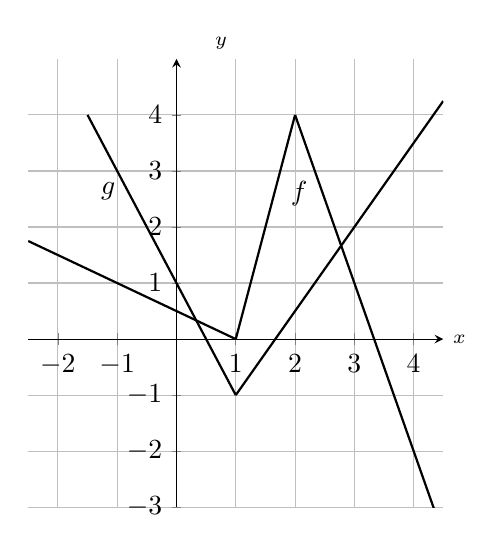
\begin{tikzpicture}
\begin{axis}[axis y line=middle,axis x line=middle, ymajorgrids=true, xmajorgrids=true, ymin=-3,ymax=5, xmin=-2.5,xmax=4.5, name=myplot, xscale=1/1.3, ytick={-3,-2,-1,0,1,2,3,4}]
\addplot [{\colorone}, domain=-1.5:1,thick] {-2*x+1}; 
\addplot [{\colorone}, domain=1:4.5,thick] {1.5*x-2.5};
\addplot [{\colortwo}, domain=-2.5:1, thick] {-.5*x+.5};
\node[label={30:{$g$}}] at (axis cs:-1.6,2.2) {};
\addplot [{\colortwo}, domain=1:2, thick] {4*x-4};
\node[label={30:{$f$}}] at (axis cs:1.6,2.1) {};
\addplot [{\colortwo}, domain=2:4.5, thick] {-3*x+10};
\end{axis}
\node [right] at (myplot.right of origin) {\scriptsize $x$};
\node [above] at (myplot.above origin) {\scriptsize $y$};
\end{tikzpicture}
\vskip .25 truecm
You can write this as 4 separately numbered problems, instead of 4 parts of one problem, if it works better that way.\\ 
(a) $(f \circ g)'(-1)$  \hskip .25 truecm (b) $(g \circ f)'(0)$ \hskip .25 truecm (c) $(g \circ g)'(-1)$ \hskip .25 truecm (d) $(f \circ f)'(4)$
}
{(a) $(f \circ g)'(-1)=6$  \qquad (b) $(g \circ f)'(0)=1$ \\
(c) $(g \circ g)'(-1)=-4$ \qquad (d) $(f \circ f)'(4)=1.5$
}
